\documentclass{article}
\usepackage[utf8]{inputenc}
\usepackage{indentfirst}
\usepackage{graphicx,animate}
\graphicspath{ {images/} }
\usepackage{array}
\usepackage[french]{babel}
\usepackage{hyperref}
\usepackage{amsmath}
\usepackage{amssymb}
\usepackage{lipsum}
\usepackage{float}
\usepackage{colortbl}
\usepackage{longtable}
\usepackage[svgnames, table]{xcolor}
\usepackage[
%	a4paper,
left=1.8cm,
right=1.8cm,
bottom=3cm,
top = 2cm,
foot=0.8cm]{geometry}
\usepackage{multicol}
\usepackage[justification=centering]{caption}
\usepackage{movie15}

\title{Projet Tweetoscope}
\author{Jérémie LEVI, Sélim OLLIVIER, Maxime RAILLAT}
\date{5 Décembre 2022}

\begin{document}
\maketitle

\section{Introduction}
Ce projet vise à implémenter une application réalisant des statistiques sur des données issues de l'API de Twitter. Le squelette de l'application étant donné, nos tâches principales consistent à intégrer une architecture Kafka dans l'application, à la conteneuriser avec Docker et Kubernetes et à mettre en place une pipeline CI/CD.

\section{Secrets and Git}
Afin de pouvoir accéder à l'API de Twitter, il nous faut disposer d'un Bearer Token. Le Bearer Token est un token unique à chaque compte développeur Twitter qui est généré pour une certaine durée. Il permet de s'authentifier de facon instantanée et par conséquent d'accéder à de nombreuses fonctionnalités Twitter.
Par exemple vous pouvez poster un Tweet, addresser un message, retrouver des adresses mails d'utilisateurs. Ce token étant lié à votre compte, il ne doit pas tomber dans les mains de n'importe qui.
Même dans un projet privé, il est fortement conseillé de ne pas push le token, et il n'est même pas envisageable de le faire pour un projet public. En effet des bots scrutent les projets publics sut Github ou Gitlab afin de récupérer un maximum d'information (identifiant, token, etc.) pour des utilisations inconnues et potentiellement malveillantes. Si vous souhaitez push votre token à tout prix, vous pouvez l'encrypter ou bien rajouter un paramètre d'entrée lors de l'exécution de votre programme. Il est également possible d'ajouter le Bearer Token en variable d'environnement dans les paramètres CI/CD du projet.

\maketitle
\section{Architectural Choices}
Pour l'élaboration de notre architecture, nous avons basé notre modèle sur la forme vue en cours avec le projet Wikimedia. Dans notre cas, nous avons un grand flux de données (Twitter), nous avons alors besoin d'absorber un grand flux de données. Pour remédier à ce problème nous pouvons mettre en place plusieurs partitions pour nos topics permettant de paralléliser le travail. \\\\
Nous devons également changer la période de rétention par défaut d'une semaine à 1 minute par exemple. Si nous ne changeons pas cette période nous allons accumuler des millions et millions de tweets avant d'arriver à saturation. Voyons maintenant en détail l'architecture de notre modèle : \\
\begin{itemize}
    \item Premièrement nous avons le module TweetProducer qui nous fournit des tweets provenant de (Internet, TestBase), nous créons alors un topic Tweet dans lequel le Producer publie les tweets.\\
    \item Deuxiemement, le module Filter qui va consommer le topic Tweet et publie dans un nouveau Topic Filter, nous gardons alors uniquement le texte des tweets qui nous intéressent. \\
    Différents filtres peuvent être appliqués : Aucun, Pays, Date ou Langue.\\
    \item Ensuite le module HashtagExtractor qui consomme les tweets publiés dans le topic Filter nous permet d'extraire les hastags de chaque tweets et de les publier dans le topic Extractor.\\
    \item Puis, le module HashtagCounter va consommer les hastags publiés dans le topic Extractor pour publier dans le topic Counter. Ce module nous sert d'aggrégateur pour compter le nombre d'occurrences de chaque hashtag. A chaque fois qu'un hashtag est consommé, une Hashmap contenant des paires (hashtag-count) est mise à jour. On sélectionne ensuite les hashtags les plus fréquents et on publie la hashmap réduite dans le topic Counter.\\
    \item Finalement le Visualizor qui va consommer le topic Counter et nous afficher les résultats sous forme d'histogramme. Nous n'avons donc pas besoin de créer un dernier topic.

\end{itemize}
\maketitle
\section{Risk Analysis / Initial Risk Analysis}
Dans notre cas il s'agit d'une chaîne en série de topics commençant par la récolte des tweets, par conséquent si l'un des topics ne remplit plus sa fonction alors nous n'aurons rien en sortie de la chaîne. Par conséquent, il faut créer un modèle le plus tolérant aux pannes possible, mais comment faire ?\\

Dans un premier temps nous augmentons le nombre de partitions permettant de répartir le flux de données important provenant de Twitter. Les partitions permettent aux utilisateurs de paralléliser les topics, ce qui signifie que les données d'un topic peuvent être réparties sur plusieurs brokers. \\
Ensuite chaque partition doit être configurée avec un total de trois réplicas. En cas de défaillance d'un topic/partition, l'un des deux répliquas deviendra la partition leader. Nous allons mettre en place trois répliquas pour prendre en charge correctement la défaillance d'un topic. \\

La question qui se pose maintenant est, comment relancer ou remettre de façon opérationnelle un répliqua tombé en panne. Grace à Kubernetes nous pouvons mettre en place une architecture capable de les relancer.
En effet chaques pod permettant le bon déroulement de l'application est contenu dans un noeud orchestré  par un Master noeud. Dans le cas où un noeud ne répond plus (heart beat = 0) au Master, celui-ci va remplacer le noeud "mort" par un noeud identique (importance des répliquas) et relancer le noeud "mort". C'est avec cette architecture que nous pensons être le plus tolérant aux pannes.

\section{Conteneurisation de l'application et déploiement sur Kubernetes}

La conteneurisation de l'application se fait en créant des fichiers Dockerfile contenant chacun une composante de l'application telle que l'HashtagExtractor ou le LangFilter. Nous avons également push ces mêmes images Docker sur le DockerHub de Maxime : \href{https://hub.docker.com/r/maxlamenace34/tweetoscope}{https://hub.docker.com/r/maxlamenace34/tweetoscope} \\

\begin{figure}[htbp]
    \centering
    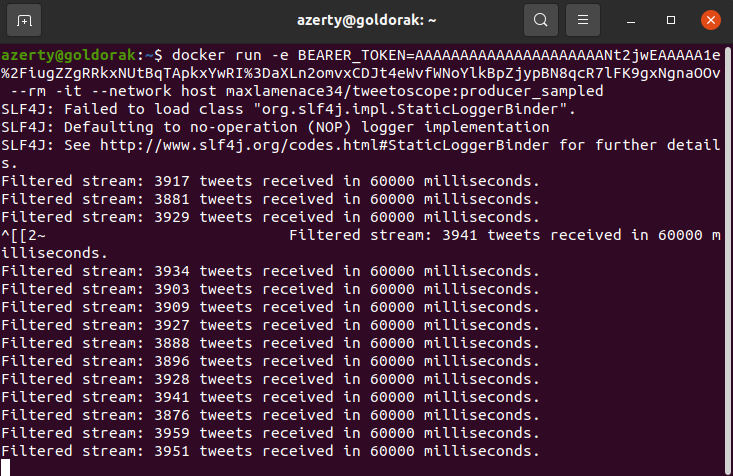
\includegraphics[scale=0.5]{images/ProducerSampled.png}
    \caption{ProducerSampled en cours d'exécution, lancé à partir d'une image Docker}
    \label{fig:1}
\end{figure}

\begin{figure}[htbp]
    \centering
    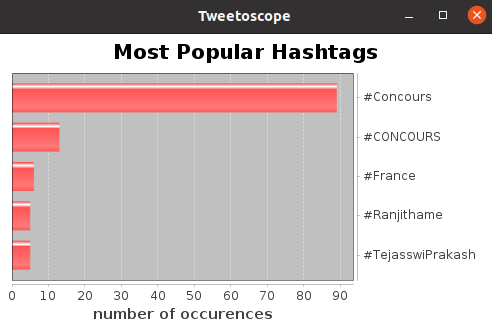
\includegraphics[scale=0.8]{images/Visualizor.png}
    \caption{Visualizor en cours d'exécution, lancé à partir d'une image Docker}
    \label{fig:2}
\end{figure}

Les différentes commandes permettant de lancer Zookeeper, Kafka puis les images Docker des composantes de l'application peuvent être trouvées dans le README.md. \\

Pour automatiser le déploiement de notre application avec Kubernetes, nous créons les fichiers $zookeeper\_kafka.yml$ et $Tweetoscope\_deployment.yml$. Le premier fichier permet de déployer Zookeeper et Kafka sur Kubernetes et le deuxième de déployer les différentes composantes de notre application sur Kubernetes. Nous avons rencontré plusieurs problèmes au niveau du déploiement sur Kubernetes : \\
\begin{itemize}
    \item Comment passer en argument une variable dans les images Docker des composantes de l'application ? \\
    En effet au départ nous passions les arguments au docker lors de son exécution avec --env variable.
    N'ayant pas trouvé d'équivalent dans kubernetes, nous avons alors décidé d'instancier cette variable dans le docker.file . Dans ce cas, la variable est directement présente dans le docker et nous pouvons exécuter le docker sans l'argument --env . 
    \\
    \item Comment faire fonctionner le Visualizor ?\\
 Lorsqu'on le lançait dans une image Docker, on obtenait des erreurs du fait que l'image Docker choisie ne puisse pas afficher de graphiques. Pour résoudre ce problème nous avons du ajouter un paquet dans le dockerfile, copier un dossier et mettre une nouvelle variable d'environnement (DISPLAY). Tout fonctionnait en local jusqu'au moment d'utiliser kubernetes. Impossible de faire fonctionner le Visualizor, nous avons donc penché pour une solution moins user friendly, print les top hashtags dans la console.
\end{itemize}

\section{Mise en place d'une pipeline CI/CD}
Nous mettons désormais en place une pipeline CI/CD via le fichier $.gitlab\textendash ci.yml$. \\

Dans un premier temps, nous avons créé un test pour le filtre DateTweetFilter, qui permet donc de tester la création d'un objet DateTweetFilter ainsi que le bon fonctionnement de sa méthode match. Nous avons ajouté ce test à la pipeline dans l'étape $test\_reports\_job$, et on publie également un rapport complet du test JUnit qu'on ajoute aux pages Gitlab du projet, accessible \href{https://maxime.raillat.pages-student.centralesupelec.fr/tweetoscope22_group-3_ollivier1_levi2_raillat3/testCoverageReport/}{ici}.\\

D'abord nous créons un stage $build\_package$ qui compile l'application et l'exporte de façon à ce qu'elle soit téléchargeable en tant qu'artefact dans un fichier $.zip$. Puis nous créons un stage $create\_docker\_image$ qui permet de créer différentes images qui contiennent chacune des composantes de l'application : $HashtagExtractor$, $LangFilter$ et $ProducerSampled$. Ces images sont créées à partir des Dockerfile correspondants. \\

 Les images Docker sont ensuite publiées dans le Containers Registry du projet sur Gitlab. Pour que l'image puisse être exécutée par les membres du projet, il nous a fallu créer un deploy token afin de pouvoir s'authentifier lorsqu'on tente d'exécuter l'image Docker depuis un terminal. \\

Enfin, nous automatisons la compilation du rapport $report.tex$ en utilisant l'image Docker $ctornau/latex$ qui est adaptée à la compilation de fichiers \LaTeX, puis nous publions le fichier pdf sur les Gitlab Pages du projet. Ce sont les stages $compile\_pdf$ et $deploy$ dans le fichier $.yml$. Les graphiques inclus dans le rapport figurent dans le dossier $/images$ du projet. \\

\section{Feedback}
Le projet s'est déroulé en trois axes principaux (Java-Kafka, Docker-Kubernetes, Pipeline-CI/CD). Cette architecture de projet nous a permis de travailler en parallèle et d'avancer de façon efficace dans les étapes. 

\subsection{Selim Ollivier}
J'ai principalement travaillé sur l'écriture du code source en Java afin d'adapter l'application à une conteneurisation et un déploiement sur Kubernetes ainsi que l'écriture et le déploiements de tests unitaires. 
N'ayant jamais réellement programmé dans un autre langage que Python, j'ai du m'adapter aux contraintes de programmation sous Java. Les débuts ont donc été quelque peu fastidieux et nous ont valu quelques temps sur StackOverFlow\dots 
Le second point dur de ce projet a pour ma part été l'adaptation des filtres : j'ai d'abord tenté d'utiliser KafkaStreams sans grand succès que ce soit avec des chaines de caractères ou des données structurées. J'ai donc basculé sur une architecture plus simple et plus facilement debuggable Producer-Consumer.
Ce projet m'a donc permis d'appréhender de nouveaux outils qui pourront peut-être m'être utiles par la suite.

\subsection{Maxime Raillat}
Je me suis principalement occupé de la partie Docker, Kubernetes, Docker-compose du projet. J'ai donc appris à utiliser de nouveaux outils très utiles pour un Data Scientist, Data Engineer. En effet, je sais maintenant déployer une environnement de travail avec Docker. Pour moi la partie la plus intéressante était Docker et Docker-compose me permettant de déployer un environnement adéquat pour un projet, un stage, etc. Kubernetes a vraiment été ma bête noire, en effet j'ai rencontré de nombreux problèmes. J'ai dû refaire tous les Dockerfiles qui étaient mal adaptés au déploiement Kubernetes. J'ai rencontré par la suite un problème d'image Docker, celui-ci ne prenait pas la dernière version enregistrée dans le Dockerhub même en précisant :latest. Il y avait aussi moins de documentation et de ressources autour de cet outil rendant l'expérience plus compliquée. Tous ces problèmes ont peut-être biaisé mon avis sur Kubernetes, j'ai alors moins apprécié cette partie du projet. Kubernetes reste tout de meme très utile pour la disponibilité, tolérance aux pannes des Dockers!

\subsection{Jeremie Levi}
J'ai principalement travaillé sur la pipeline CI/CD du projet et un peu sur le déploiement sur Kubernetes avec les images Docker. Pour l'intégration des images Docker des composantes de l'application, il s'agissait surtout de trouver des images adaptées, par exemple pour le Visualizor on ne pouvait pas simplement utiliser l'image Docker $openjdk$ car elle ne permettait pas d'afficher l'histogramme; de même pour la compilation du rapport en pdf, ce n'était pas évident de trouver une image sur Dockerhub qui prenne en charge des graphiques dans la compilation du fichier $.tex$. J'ai également fait face à un bug assez embêtant sur Gitlab, lorsqu'on a beaucoup d'artefacts de jobs qui se cumulent, l'espace de stockage du projet augmente énormément et on s'est retrouvé avec presque 10 Go alors que les fichiers en eux-mêmes et les images Docker ne dépassent pas la centaine de Mo en tout.
\end{document}
